\documentclass[a4paper, 10pt, final, garamond]{book}
\usepackage{cours-preambule}

\titleformat{\item}{}{\arabic{item})}{.5em}{}{}
\titleformat{\subitem}{}{\arabic{item}) \alph{subitem} --}{.5em}
{}{}

\makeatletter
\renewcommand{\@chapapp}{Devoir surveill\'e -- num\'ero}
\makeatother

\begin{document}
\setcounter{chapter}{0}

\chapter{Commentaires sur le DS n\degree01}

% \begin{tcb}*(prop)"bomb"{Malus}
% 	\begin{minipage}{0.50\linewidth}
% 		\begin{itemize}
% 			\item N~: numéro de copie manquant~;
% 			\item E~: manque d'encadrement des réponses~;
% 			\item M~: marge non laissée ou trop grande~;
% 			\item V~: confusion ou oubli de vecteurs~;
% 			\item C~: copie grand carreaux~;
% 			\item A~: application numérique mal faite~;
% 		\end{itemize}
% 	\end{minipage}
% 	\begin{minipage}{0.50\linewidth}
% 		\begin{itemize}
%       \item P~: prénom manquant~;
% 			\item Q~: question mal ou non indiquée~;
% 			\item H~: homogénéité non respectée~;
%       \item U~: mauvaise unité (flagrante)~:
%       \item S~: chiffres significatifs erronés.
% 		\end{itemize}
% 	\end{minipage}
% \end{tcb}

\section{Commentaires généraux}

Bravo pour ce premier DS. Les bases sont globalement solides, le cours est
connu. Il reste justement à réussir à se détacher du cours et traiter les
problèmes. La moyenne a été placée à 11.

Par contre, un nombre incalculable de malus. \textbf{Suivez les consignes}~: si
vous répondez à une question, il faut le numéro, même si c'est sur une annexe.
Le numéro des \textbf{copies} n'est pas le numéro des \textbf{pages}.

\begin{tcb}[bld,cnt,fontupper=\Large](impo){Lentilles}
Les lentilles divergentes n'ont \textit{rien} de spécial~!
\end{tcb}
Trop de résultats faux basés sur des «~(lentille divergente)~», alors que
\textbf{rien} ne justifie un traitement différent. Reprenez les bases sur les
lentilles.

\begin{center}
	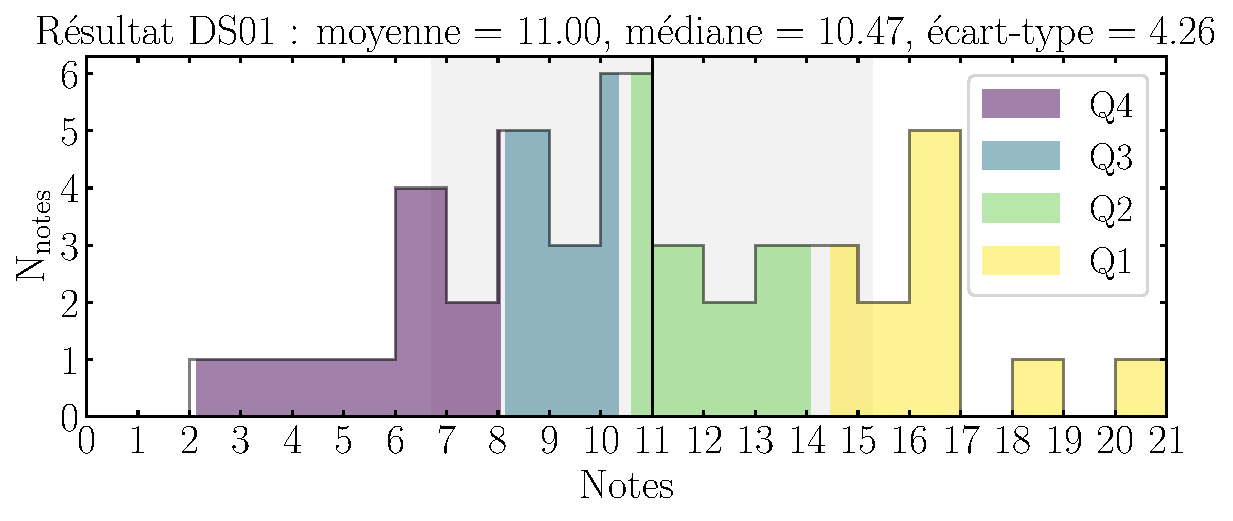
\includegraphics[width=.7\linewidth]{DS01_rslt.pdf}
\end{center}

\exercice[32]{Lentilles minces}
\begin{enumerate}
  \nitem{8} Globalement ok. Pensez bien à écrire complètement votre expression
    littérale avant de l'encadrer/la calculer~:
    \[
      \frac{1}{\OAp} = \frac{1}{\OA} + \frac{1}{f'}
      \qou
      \OAp = \left[\frac{1}{\OA} + \frac{1}{f'}\right]^{-1}
    \]
    ne sont pas des réponses satisfaisantes.
    \smallbreak
    \textbf{Attention}, $\gamma \neq G$~!!
    \nitem{5} Vous ne pouvez pas dire que vous calculez le grandissement si vous
    utilisez $\gamma = \frac{\ABp}{\AB}$ que vous mesurez sur votre schéma…
    \nitem{5} RAS.
    \nitem{3} Soyez attentif-ves. N'ayez pas une mémoire d'éphémère~: les
    questions d'un énoncé se suivent et souvent à raison. Il faut savoir prendre
    du recul et noter ce que vous venez de faire.
    \nitem{5} C'est fâcheux, mais beaucoup de tentatives de preuves ne sont pas
    recevables. Trois schémas avec l'objet avant, sur et après le foyer objet ne
    consitute pas une démonstration. Il faudrait pour ça montrer que toutes les
    positions avant le foyer son similaires, et de même pour les positions
    après. J'ai accepté les justifications concernant la nature divergente ou
    convergente d'un faisceau incident et la nature de la lentille (quand
    c'était bien fait).
    \nitem{4} Idem.
    \nitem{2} Idem.
\end{enumerate}

\exercice[48]{Instruments à l'infini}
\begin{enumerate}
  \nitem{4} Vous avez très bien appris le cours, mais presque trop~! Il faut
  établir le fait que les foyers soient confondus. Et surtout, \textbf{le
  résultat ne dépend pas de la nature des lentilles}~!! Trop de $\obar{\rm
  O_1O_3} = f_1' - f_3'$ parce que «~lentille divergente~»… Ça n'a rien à voir.
  \nitem{3} Aléatoire.
  \nitem{3} Indiquez l'annexe~! RAS.
  \nitem{4} Et \textsc{Newton}~? Pas une bonne réponse avec \textsc{Newton}.
  \nitem{5} Très peu de représentation optiques, et aucune bonne réponse ici. À
  reprendre.
  \nitem{6} Idem, à justifier. \textit{Afocal} signifie bien «~sans foyer~»~: il
  faut bien distinguer les foyers des sous-composants et les foyers du système
  complet. On ne peut définir un foyer pour un système afocal (revoir
  définition).
  \nitem{6} Il était attendu de faire un schéma de la lunette, pas des
  conditions de \textsc{Gauss}. J'ai compté les points pour un schéma fait
  question 8.
  \smallbreak
  Conditions de \textsc{Gauss} mal comprises, confondues avec leurs conséquences
  (stigmatisme, aplanétisme).
  \nitem{5} Ici aussi, vous avez trop le cours~: le résultat de grossissement
  n'est pas connu. Il se démontre. Et si vous prétendez le connaître, alors
  connaissez-le…
  \smallbreak
  Je n'ai pas commenté l'absurdité de trouver des grossissements de \num{0.02},
  \xul{pour cette fois}. Soyez critiques~!
  \nitem{2} RAS
  \nitem{2} Un manque certain de démonstration.
  \nitem{2} Attention aux CS (chiffres significatifs).
  \nitem{4} Il fallait remarquer la monture… RAS.
  \nitem{2} Vu chapitre 1~: dispersion (et pas diffraction).
\end{enumerate}

\setcounter{section}{0}
\prblm[30]{Gemmes}
\begin{enumerate}
  \nitem{8} Plein de points à prendre ici, mais encore faut-il savoir les
  prendre. Il peut y avoir réflexion totale car un rayon s'écarte de la normale
  en passant dans un milieu moins réfringent, on peut donc avoir des rayons
  réfractés inexistant.
  \nitem{2} Dispersion.
  \nitem{4} De même, les questions se suivent et avec raison. Certains rayons
  ont $i<i_{l}$…
  \nitem{1} Attention CS.
  \nitem{3} Faire des comparaisons physiques. «~Ma calculatrice me dit
  "indéfini" donc ça ne marche pas~» n'est pas un argument valide. «~L'indice de
  la moissanite étant supérieur à celui du verre, il ne peut y avoir réflexion
  totale~» l'est beaucoup plus.
  \nitem{2} Masse volumique n'est pas le poids…
  \nitem{6} Très peu faites. Il faut avoir le réflexe des rayons qui se
  rapprochent ou s'écartent.
  \nitem{4} RAS.
\end{enumerate}

\prblm[32]{Gobelet}
\begin{enumerate}
	\nitem{3} Confusions entre conditions et conséquences.
  \nitem{2} RAS.
  \nitem{2} RAS.
  \nitem{4} Le schéma n'étant pas à l'échelle, vous ne pouvez pas tracer les
  triangles qui vous arrangent pour le calcul. Il faut tracer des triangles qui
  respectent la géométrie du problème.
  \nitem{7} RAS.
  \nitem{3} Erreur d'énoncé. Points comptés pour construction cohérente.
  \nitem{5} Non traitée.
  \item[8+)]{\gpts{6}} Non traitées.
\end{enumerate}

\end{document}
